\documentclass[a4paper,final]{article}

\usepackage{a4wide}

% Language and encoding
\usepackage[utf8]{inputenc}
\usepackage[T1]{fontenc}
\usepackage[english]{babel}
\usepackage[protrusion=true,expansion=true]{microtype} % better typography

% Math
\usepackage{amsmath,amssymb,amsfonts,amsthm}
\usepackage{mathabx}

\newtheorem{thm}{Theorem}[section]
\newtheorem{defn}{Definition}[section]

\newcommand{\bbN}{\mathbb N} %the natural numbers
\newcommand{\bbZ}{\mathbb Z} %the integers
\newcommand{\bbQ}{\mathbb Q} %the rational numbers
\newcommand{\bbR}{\mathbb R} %the real numbers
\newcommand{\bbC}{\mathbb C} %the complex numbers

% Graphic stuff
\usepackage[pdftex]{graphicx}
\usepackage[usenames,dvipsnames,table]{xcolor}
\definecolor{shade}{RGB}{235,235,235}
\usepackage[pdftex,colorlinks=true]{hyperref}
\hypersetup
{
    bookmarksnumbered,
    linkcolor=RoyalBlue,
    anchorcolor=RoyalBlue,
    citecolor=RoyalBlue,
    urlcolor=RoyalBlue,
    pdfstartview={FitV},
    pdfdisplaydoctitle
}

% Tables
\usepackage{booktabs}
\usepackage[hang,small,bf]{caption}

% Debug, etc.
\usepackage{todonotes}

% Computer science stuff
\usepackage{clrscode3e}
\usepackage{verbatim}
\newcommand{\mono}[1]{{\ttfamily#1}}
\usepackage{listings}
\lstset
{
    tabsize=2,
    numbers=left,
    breaklines=true,
    backgroundcolor=\color{shade},
    framexleftmargin=0.05in,
    basicstyle=\ttfamily\small,
    numberstyle=\tiny,
    keywordstyle=\color{RoyalBlue},
    stringstyle=\color{Maroon},
    commentstyle=\color{ForestGreen},
    language=Matlab
}



\usepackage{subfig}
\newcommand{\subfigureautorefname}{\figureautorefname}


\title{Principles of Computer Systems Design -- Assignment 1}
\date{\today}
\author{Daniel Egeberg \and Søren Dahlgaard}

\begin{document}

\maketitle

\section{Exercises}

\subsection*{Question 1}
Our scheme is very simple: First calculate which machine to contact, and what
the memory address is on that machine. Second contact the machine over ethernet
(i.e.\ some local LAN).

We make the assumption, that we are aware of how much memory each individual
machine has when creating the scheme. Two cases then present themselves:
\begin{enumerate}
    \item Each machine has the same amount of memory it is very easy to
        calculate the machine and address using $a\mod m$ and
        $\lfloor a/m \rfloor$, where $a$ is the address, and $m$ is the amount
        of memory.
    \item If this is not the case, it is slightly more complicated. One way to
        handle this is to keep an array in the translation code, which contains
        the accumulated sizes, and then doing a binary search on this array to
        find the machine. E.g.\ if machine $0$ and $1$ have $2$ GB of memory and
        machine $2$ and $3$ have $4$ GB of memory, the array would contain
        the values $[0, 2\cdot 10^9, 4\cdot 10^9, 8\cdot 10^9]$. We then simply
        do a binary search for the biggest number in the array, that is smaller
        than the sought address $a$. Then calculating the local address on the
        machine is trivial. This adds a $\log$ factor of the number of
        machines, but this number will never be big enough to be a dominating
        factor.
\end{enumerate}

To have the API look as similar to the one for local memory, we limit
$\proc{Read}$ and $\proc{Write}$ to only accessing one byte at a time. See the
pseudocode below. The pseudocode is for the one-size memory version, but the
other one is almost just as simple. Assume $m$ to be some global constant.

\begin{codebox}
    \Procname{$\proc{Read}(a, p)$}
    \li $d\gets a\mod m$
    \li $a2\gets \lfloor a/m \rfloor$
    \li $p\gets\proc{Send}(d, \const{read}, a2)$
\end{codebox}

Here $\proc{Send}$ is some generic network procedure, that sends the command
$\const{read}$ to the machine at $d$ with parameters $a2$. We assume $p$ to
be some reference to store the received data in. The pseudocode
is the same for $\proc{Write}$ except the $\proc{Send}$ call will send the
command $\const{write}$ instead and takes an extra parameter -- the value to
write.

Read/write operations to regular main memory is clearly atomic, as it is
performed with a single hardware instruction -- although the electric signal
could end up being corrupted, this is \emph{extremely} unlikely. Since our
method only writes one byte at a time, and this is done using one instruction
in the receiving machine, it is clear that our method is atomic as well. We do
this because we want the API to be as similar to performing the operations on
regular main memory as possible.


\subsection*{Question 2}

We have filled the table using values from \cite{WikiSSDHDD}, \cite{WikiDRAM}
and \cite{PowerConsump}. Prices and capacities have been found using
\url{www.edbpriser.dk}. Note that access time is for everything -- this
includes rotational latency and seektime for HDDs. We have not split into read
and write, but rather split into Access time and transfer rate, as we believe
this to be more relevant. For reliability we considered how long a unit is
expected to last. For instance, the moving parts of the HDD is subject to wear
and tear and thus will wear down. The transfer rates have not been normalized,
but are with different units -- we assume that $1\text{ Word} = 4\text{ Bytes}
= 32\text{ bits}$. For sizes we have listed commonly available size only. For
example, even though SSDs of more than $2$ TB are available, these are not
common at all.

\begin{table}[htbp]
    \centering
    \rowcolors{1}{white}{shade}
    \begin{tabular}{ l | p{.2\textwidth} | p{.2\textwidth} | p{.2\textwidth} }
        \toprule
        & \textbf{HDD} & \textbf{SSD} & \textbf{RAM} \\
        \midrule
        Access time (total) & 12ms & 0.1ms & 33.75ns \\
        Transfer rate & 1023 Mbit/s & 100 to 600 MB/s & 1600MWord/s \\
        Capacity (common) & Up to $4$TB & Up to $512$GB & Up to $32$GB \\
        Cost per GB & $0.4$ DKK & $5$ DKK & $32$ DKK \\
        Reliability
            & Moving parts subject to wear and tear
            & Only allows limited number of writes before fail (typically many years under normal use)
            & Good \\
        Power consumption & $2$ to $5$ W & $1/3$ of HDD & $5$ to $15$ W \\
        \bottomrule
    \end{tabular}
\end{table}

Which kind of storage to use for our abstraction depends a lot on how we wish
to use the abstraction. We see it as a huge memory abstraction used in a LAN
setting, where the ethernet connection is very fast. In this case HDDs would
certainly incur a too big latency overhead to be practical. Also, since writes
to disks like HDDs and SSDs are page based we cannot ensure the atomicity we
wish to keep our abstraction as close to working with normal memory as we can.
Thus we would only use RAM.


\subsection*{Question 3}
\begin{description}
\item [a)]\ \\
Concurrency does not have a big impact on latency. This is because each
instruction is not performed faster, but rather several instructions are
performed at once. This gives bigger throughput, but not better latency. In
fact the overhead incurred by the concurrent requests is more likely to have
a slight negative effect due to more bookkeeping. Also some requests may need
to acquire locks to access shared resources, which increases the latency of
the individual request.

\item [b)]\ \\
Batching and dallying are two entirely different things. The only thing they
have in common is that they can be used to fight bottlenecks. Batching is when
you group several requests together before sending them, to avoid the setup
overhead. Dallying is when you don't send a request at all because it might
not be needed.

An example of batching could be retrieving multiple records from a database
at once, by e.g.\ performing an SQL select of all items with id between $10$ and
$20$, rather than retrieving one record at a time.
An example of dallying could be in cache, where a memory write is not written
to main memory immediately when issued, but is delayed until the cache line
has to be replaced.
\item [c)]\ \\
Caching is clearly an example of fast path optimization. When working with
memory it is very common to work with the same area a lot, e.g.\ reading a value
adding something to it, and storing it again or searching through an array.
A cache optimizes for this, and thus the common case by providing a fast path
to this memory once it has been referenced once.
\end{description}


\subsection*{Question 4}
\begin{description}
\item [a)]\ \\
    Assuming that we are testing the L1 cache, we need to know the size of a
    cache line. We could just read the same memory address a lot of times, but
    this is probably not too good, as we will run into too many different
    optimizations in both software and hardware. Rather, we want to read the
    same few values. Since we cannot decide how cache lines are replaced it
    is very hard to utilize the entire cache to be sure that we avoid such
    optimizations. One way to test the bandwidth would be to read some $64$
    consecutive bytes (the size of a typical cache line) into the cache and
    then access these over and over. We must of course turn off all compiler
    optimizations before doing this.

    By performing say, $2^{30}$ reads we can see how long time it takes to do
    this, and obtain how many seconds are needed to read one GB\@. This does,
    however not take advantage of any parallelism in the cache, so reading
    words or dwords may be the better option for real effective bandwidth.

    We use cache reads, as these cause less delay then reads from an
    instruction cache, but more than a write miss (due to dallying). This
    gives a good midway.
\item [b)]\ \\
    It is quite to ensure, that all reads are cache misses. This depends
    heavily on the replacement strategy used by the CPU cache, as well as which
    type of cache it is (direct-mapped, set-associative, full associative,
    etc.). One way to completely avoid this issue, is to only access one
    element per possible cache line, flushing the cache when the CPU begins.
    If we assume a $64$ byte cache line size, we could access every $64$th
    byte of the memory. This way, we can probably not perform $2^{30}$ reads
    unless we have a lot of memory. Instead, we could read some $100$ MB and
    measure the time for these. To get the bandwidth.
\end{description}


\section{Implementation}

\subsection*{Question 1}
Which RPC style to use depends a lot on what the key-value store is supposed
to be used for. If it is to be used in potentially life critical operations
we would need to use exactly-once or in some cases at-least once. For a simple
web service it would probably be sufficient to use an at-most once policy.
Then the user can handle the case of a timeout himself and some times he might
have to resend a request if it is of high importance.

\subsection*{Question 2}
The main parts of our implementation are described below:

\begin{description}
    \item [\mono{StoreImpl}]\ \\
        Our Store implementation is just a wrapper on top of the provided
        \mono{MemoryMappedFile} using a \mono{RandomAccessFile}.
    \item [\mono{IndexImpl}]\ \\
        Out Index implementation consists of two parts: A \mono{TreeMap} that
        contains the position and size of each key in the store, and a list
        of free blocks of memory in the file. This way we get a
        \mono{malloc}-like functionality on the store, such that we can reuse
        space when keys are removed, by adding the block back into the list,
        possibly merging it with existing ones. All operations are simply done
        by looking the key up in the \mono{TreeMap} and then either reading or
        deleting the position in the store. All the operations are without any
        form of synchronization, as we handle this in the
        \mono{KeyValueBaseImpl}.
    \item [\mono{KeyValueBaseImpl}]\ \\
        The key-value implementation is really juts a glorified wrapper around
        \mono{IndexImpl}, which also handles synchronization, by using a
        \linebreak
        \mono{ReentrantReadWriteLock}. We do not use per-key locks, as we like
        the \mono{KeyValueBaseImpl} to handle locks. It would, however, be easy
        to change this and let the Index handle a lock per key. This, does
        however add some requirements on \mono{bulkPut} and \mono{atomicScan},
        as these would have to acquire all locks in the beginning to ensure
        atomicity. This could potentially incur deadlocks, unless keys are
        acquired in a controlled fashion (i.e.\ increasing by keys).
        The \mono{init} function of the class reads in the keys one by one
        and adds them via the index. The only thing we need to consider here,
        is that a key may span multiple lines, but since these are sorted it
        is trivial to handle.
\end{description}

We took the decision to implement \mono{ValueImpl} using integers to make it
work with the web service, which cannot handle generic types. This also
simplifies many of our other classes. Our serialization is done by simply
storing each integer as four bytes, which makes the whole process very easy.

We additionally had to create a class \mono{KeyValueBaseService}, which wraps
\mono{KeyValueBase}, to make it work with the web service and JAX-WS. This
class encapsulates a lot of types because interfaces and collections can't be
used with JAX-WS. Instead we use plain arrays for return types in scan
operations and wrap the input types in our own classes. All the packing in
and out of wrappers is done by \mono{KeyValueBaseService}, to keep the
interface of the \mono{KeyValueBase} consistent with the assignment.

\subsection*{Question 3}

We have created a class \mono{test.Main} that tests the individual procedures
in our key-value store. It first initializes the service using a data file.
Using this we can test \mono{read} by reading keys we know already exist. We
can then \mono{insert} and \mono{update} new keys and read them similarly to
ensure that we get the expected values back. \mono{bulkPut} and \mono{scan} are
tested in a similar fashion. Concurrency is tested by starting multiple new
threads and having them \mono{update} and \mono{read} values with artificial
waiting times between 100~ms and 1500~ms induced by calling Java's
\mono{Thread.sleep}.

\subsection*{Question 4}
The parameters are discussed in the following list. We only consider the
parameters noted in the assignment.

\begin{description}
    \item [Number of Clients] influence the throughput greatly, as the web
        service is able to handle concurrent requests. Note however, that it
        might actually decrease both throughput and increase latency due to
        the mix of operations (see below).
    \item [The hardware] greatly influences latency, as it decides how much of
        the memory-mapped file can remain in the main memory, and thus how
        long it takes to read/write requests. Also, more processors will
        allow for more concurrent requests, thus increasing the throughput.
    \item [The size of the dataset] influences latency in the same way as the
        hardware does. If the dataset is huge -- less of it can be in main
        memory, and thus response time will increase.
    \item [Mix of operations] Because we employ CREW (concurrent read,
        exclusive write) locking, write operations greatly increase latency
        of read operations and decreases the throughput.
\end{description}


\subsection*{Question 5}
As mentioned in the previous question, we expect the number of clients to
increase the throughput, as long as the hardware has cores/hardware threads
to support this. As such, we expect the throughput to increase almost linearly
until there are as many clients as the service can execute simultaneously
threads. The latency shouldn't be effected much unless the clients are
performing a lot of writes, which will block out other requests.

\subsection*{Questions 6 and 7}

We tested the service running on a single Lenovo Thinkpad T420 with the
following specifications:

\begin{itemize}
    \item Intel Core i5-2520M CPU @ 2.50GHz
    \item 8 GB RAM
    \item 256 GB SSD
\end{itemize}

The service's storage was set to 10 GB and initialized with the LiveJournal
data set. We spawned up to 50.000 threads \mono{read}ing keys drawn from the
Zipf distribution with a maximum value of 1000. The results in throughput and
latency can be seen in \autoref{fig:experiments}.

\begin{figure}[h]
    \centering
    \subfloat[Latency]{\label{fig:latency}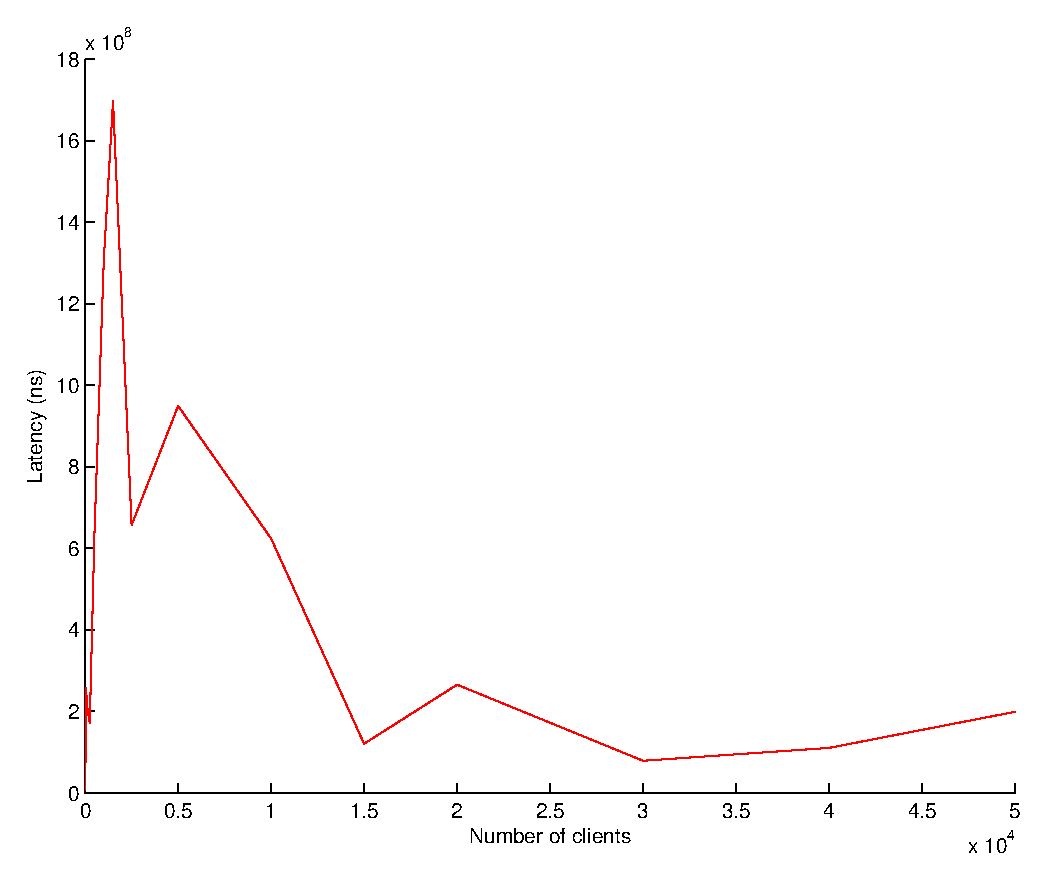
\includegraphics[scale=.4]{latency}}
    \subfloat[Throughput]{\label{fig:throughput}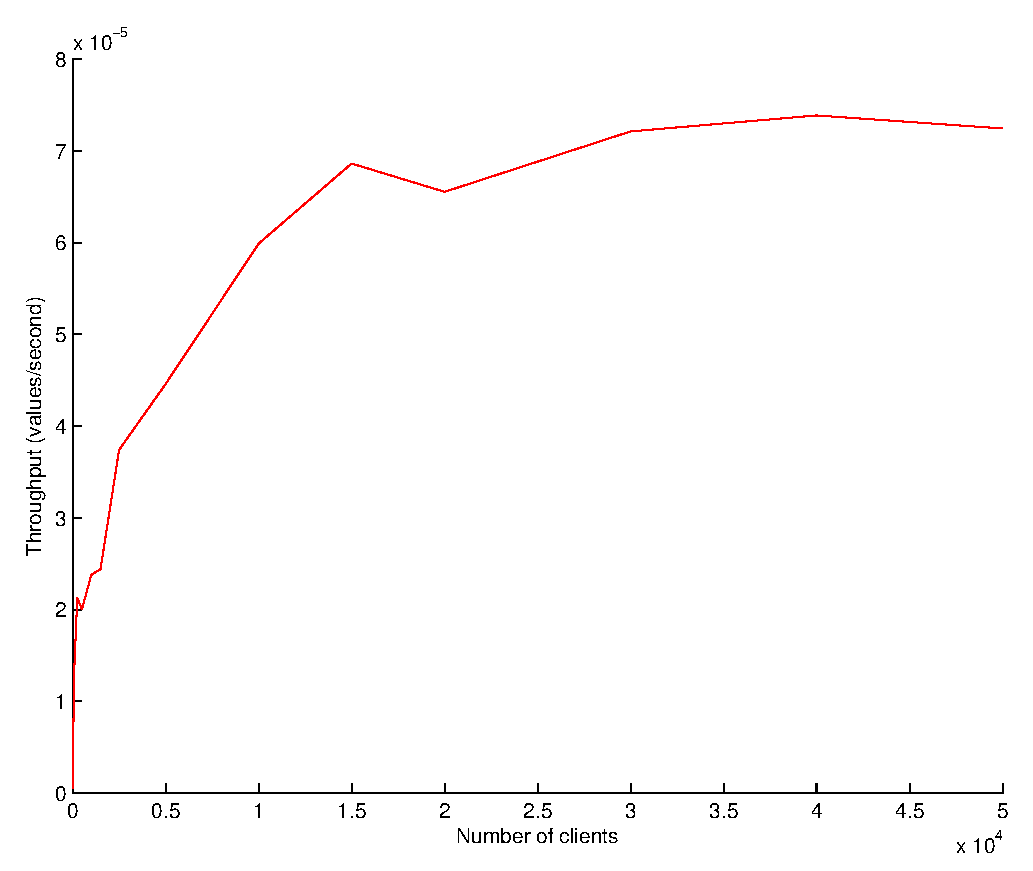
\includegraphics[scale=.4]{throughput}}
    \caption{Experiment results}
    \label{fig:experiments}
\end{figure}

The computer we tested on has 4 cores, and as we see in \autoref{fig:latency},
the graph flattens out because the amount of concurrent requests we can handle
is limited by the cores. \autoref{fig:latency} shows a more or less flat graph,
meaning that the number of concurrent clients doesn't influence the throughput
in no significant way. The spikes in the start may be due to overhead in the
measuring, as after 500 clients it drops and becomes stable.

The Zipf distribution samples were generated by the Apache Common Math library.

\subsection*{Question 8}
We would definitely like to perform some tests on a computer with much
less/more memory to see the latency de-/increases we expect from the
memory mapped file response times. The same result should be obtainable by
using a smaller/bigger dataset.

The experiment from question 5 also only uses \mono{read} operations, which
are by far the fastest. We would like to see the effect of adding \mono{write}
operations to the mix -- e.g.\ having every $n$th operation as a write for
different $n$, to see how much concurrency we can get out of the reads while
they have to wait once in a while. This should decrease throughput, and
increase the latency of \emph{some} of the read operations.

\subsection*{Question 9}
As already noted, both methods had to be fitted heavily to work with JAX-WS\@.
This means, that the interface for the end-user (not the
\mono{KeyValueBaseImpl}) has changed a bit to allow the user to pass a
collection over JAX-WS\@. Since we don't use per-key locks, \mono{atomicScan}
simply acquires the read lock and then calls \mono{scan}. If one read fails
the user will get an exception, and thus the entire procedure is atomic.

Our \mono{bulkPut} is implemented by acquiring the write lock and then
inserting or updating the entries. While doing so, it keeps a log of all the
changes it has made, and tries to restore these if an update fails. This
almost ensures atomicity, but has a few flaws. First of all, the log is kept
in memory, so if one tries to update the entire store, the log will be too
big, and the system is likely to crash. Also, if one of the rollback writes
fail, we do nothing, as this is a slippery slope. In the general case it
should work well, though.


\begin{thebibliography}{9}
\bibitem{PowerConsump}
    Tom's Hardware,
    \emph{Component Power Requirements},
    \url{http://www.tomshardware.com/reviews/power-saving-guide,1611-4.html},
    2007.

\bibitem{WikiDRAM}
    Wikipedia,
    \emph{Dynamic random-access memory},
    \url{http://en.wikipedia.org/wiki/Dynamic_random-access_memory},
    2012.

\bibitem{WikiSSDHDD}
    Wikipedia,
    \emph{Comparison of SSD with HDD},
    \url{http://en.wikipedia.org/wiki/Solid-state_drive#Comparison_of_SSD_with_hard_disk_drives},
    2012.
\end{thebibliography}


\end{document}
